\documentclass[11pt,letterpaper]{report}

\author{Mendoza-Cortes Group}
\title{Machine Learning Methods in Sciences}
\usepackage{fancyhdr}
%\lhead{Report}
\rhead{Mendoza-Cortes Group}
%\rhead{\today}
\headheight 35pt 

%%%%%%%%%%%%%%%%%%%%%%%%%%%%%%%%%%%%
% Begin Load Packages %%%%%%%%%%%%%%%%%%%%%%%%
%%%%%%%%%%%%%%%%%%%%%%%%%%%%%%%%%%%%

\usepackage{listings}
\usepackage{etex}
\usepackage{graphicx}
\usepackage{booktabs}
%\usepackage[flushleft]{threeparttable}
\usepackage[margin=1.0in]{geometry}
\usepackage{caption}
\usepackage{subcaption}
%\usepackage{titlesec}
\usepackage{hyperref}
\hypersetup{colorlinks=true,  % false: boxed links; true: colored links
	linkcolor=blue,   % color of internal links
	urlcolor=magenta, % color of external links
	citecolor=blue    % color of links to bibliography
}

% Package for chemistry formulas %%%%%%%%%%%%%%%%%%%%%%%%
\usepackage[version=3]{mhchem}

%%%%%%%%%%%%%%%%%%%%%%%%%%%%%%%%%%%%
% End Load Packages %%%%%%%%%%%%%%%%%%%%%%%%%
%%%%%%%%%%%%%%%%%%%%%%%%%%%%%%%%%%%%


%%%%%%%%%%%%%%%%%%%%%%%%%%%%%%%%%%%%
% Begin Extra Functionality %%%%%%%%%%%%%%%%%%%%%%
%%%%%%%%%%%%%%%%%%%%%%%%%%%%%%%%%%%%
% Adjust sticky notes
\usepackage{xargs} 
\usepackage[colorinlistoftodos,prependcaption,textsize=tiny]{todonotes}
\newcommandx{\you}[2][1=]{\todo[linecolor=green,backgroundcolor=green!25,bordercolor=green,#1]{#2}}
\newcommandx{\jose}[2][1=]{\todo[linecolor=red,backgroundcolor=red!25,bordercolor=red,#1]{#2}}
\newcommandx{\both}[2][1=]{\todo[linecolor=blue,backgroundcolor=blue!25,bordercolor=blue,#1]{#2}}
%%%%%%%%%%%%%%%%%%%%%%%%%%%%%%%%%%%%
% End Extra Functionality %%%%%%%%%%%%%%%%%%%%%%%
%%%%%%%%%%%%%%%%%%%%%%%%%%%%%%%%%%%%


%%%%%%%%%%%%%%%%%%%%%%%%%%%%%%%%%%%%
%Begin Table of contents extras. This will put the title Page on top of the table of contents
%%%%%%%%%%%%%%%%%%%%%%%%%%%%%%%%%%%%
\addtocontents{toc}{~\hfill\textbf{\large Page}\par}
\addtocontents{lof}{~\hfill\textbf{\large Page}\par}
\addtocontents{lot}{~\hfill\textbf{\large Page}\par}
%\addcontentsline{toc}{section}{Title}
%%%%%%%%%%%%%%%%%%%%%%%%%%%%%%%%%%%%
% End Table of contents extras
%%%%%%%%%%%%%%%%%%%%%%%%%%%%%%%%%%%%



%%%%%%%%%%%%%%%%%%%%%%%%%%%%%%%%%%%%
% Begin the Actual Document %%%%%%%%%%%%%%%%%%%%%
%%%%%%%%%%%%%%%%%%%%%%%%%%%%%%%%%%%%


\begin{document}
	
	\setcounter{page}{1}
	\pagenumbering{roman}
	\thispagestyle{empty}
	
	
	
	
	\maketitle
	
	\newpage
	
	\tableofcontents
	\addcontentsline{toc}{chapter}{List of Contents} 
	
	\listoftables
	\addcontentsline{toc}{chapter}{List of Tables}
	
	\listoffigures
	\addcontentsline{toc}{chapter}{List of Figures}
	
	
	\clearpage
	\newpage
	\pagenumbering{arabic}
	\setcounter{page}{1}
	\pagestyle{fancy}
	
	%*************************************************************** %
	% % % % % % % % % % % % % % % % % % % % % % % % % % % % % % % % %
	%*************************************************************** %
	%*************************************************************** %
	% % % % % % % % % % % % % % % % % % % % % % % % % % % % % % % % %
	%*************************************************************** %
	%*************************************************************** %
	% % % % % % % % % % % % % % % % % % % % % % % % % % % % % % % % %
	%*************************************************************** %
	
	%%%%%%%%%%%%%%%%%%%%%%%%%%%%%%%%%%%%
	% Begin Chapter Document %%%%%%%%%%%%%%%%%%%%%
	%%%%%%%%%%%%%%%%%%%%%%%%%%%%%%%%%%%%
	
	
	\begin{abstract}
		The following guide is intended for non CS majors that would like to use  Machine Learning on their field. It contains applications to Art, Engineering, Physics, Medicine and Chemistry.
	\end{abstract}
	
	\clearpage
	\newpage
	\chapter{Introduction and Background}
		What machine learning algorithms should you use? There are several methods that take your data and automatically evaluate algorithms on it. Those methods don't tune the algorithm parameters or don't use the recent technology. In this notes we aim to give several examples of algorithms and applications to help you identify the one suitable for your problem in deep enough to explaining how to tune them.
	
	Software required:
	This guide will require a basic knowledge of python 3, we recommend to install it with Anaconda. We also have notebooks that serve as an introduction to Python.
	Half of the lectures use  Sklearn. ``Neural Networks'' contain a lecture on Keras. For the advanced parts we have lecture ``Pytorch Tensorflow'' where we introduce both tools.
	
	
	
	%%*************************************************************** %
	%% % % % % % % % % % % % % % % % % % % % % % % % % % % % % % % % %
	%%*************************************************************** %
	%%*************************************************************** %
	%% % % % % % % % % % % % % % % % % % % % % % % % % % % % % % % % %
	%%*************************************************************** %
	%%*************************************************************** %
	%% % % % % % % % % % % % % % % % % % % % % % % % % % % % % % % % %
	%%*************************************************************** %
	%
	%%%%%%%%%%%%%%%%%%%%%%%%%%%%%%%%%%%%%
	%% Begin Chapter Document %%%%%%%%%%%%%%%%%%%%%
	%%%%%%%%%%%%%%%%%%%%%%%%%%%%%%%%%%%%%

	\subsection{Preprocessing Data}
	Most of the time we are in the supervised case, so we assume that you have measured data, for each value you have a label. Perhaps you have a list of diagnosis of patients and the label is 1 if they developed Cancer or 0 otherwise, or you have a lot of molecular configuration of materials and the label is the capacity. We wonder if we  can we make reasonable predictions for the labels of new, unseen data values?
	
	 A big part of the performance of a machine learning algorithm relies on the data. If we don't have enough data, or if it is biased, the algorithms will reflect that in their classification. For example, we worked with certain 3D-scanners until we realized they don't work with people of color. The community on twitter suggested that it was an illumination issue but deciding that the algorithm is ready after it performs well on white people while not caring about the results on people of color is a choice that makes the algorithm biased.
	 
	 With enough data, all algorithms suited for the task have similar performance. 
	 
	  In principle you should never work on data that was collected for a different experiment. Since data is collected by humans, you should always look for mistakes by cleaning and preprocessing the data. The  notebook `` First Machine Learning Notebook'' is an excellent guide on data analysis followed by ``Higher Dimensions'' which explains the curse of dimensionality and gives an introduction to higher dimensional geometry. After some experience, we recommend  the notebooks `` The Cocktail Party Problem'' which requires more math and familiarity with programming. As preprocessing we consider the problem of finding a good representation of our data that helps with the classification process. We will use Taylor series to Build such a map, we know that for a convex function the Hessian is positive definite. So one strategy would be to add any positive definite quadratic form as the non linear part of our map, in ``Information Geometry and Dynamic Entropy'' we review the implications of this process for information theory.
 	
 	
	\subsection{SVC}
	Imagine a factory environment; heavy machinery under constant surveillance of some advanced system. The task of the controlling system is to determine when something goes wrong; the products are below quality, the machine produces strange vibrations or something like a temperature that rises. It is relatively easy to gather training data of situations that are OK; it is just the normal production situation. But on the other side, collection example data of a faulty system state can be rather expensive, or just impossible. If a faulty system state could be simulated, there is no way to guarantee that all the faulty states are simulated and thus recognized in a traditional two-class problem. We will se how SVM can solve this problem.
	
	\begin{figure}[h!]
		\centering
		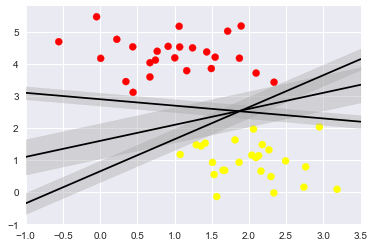
\includegraphics[width=0.45\linewidth]{figures/svcl.png}
		\caption{}
		\label{fig:lines}
	\end{figure} 
	
	Let's return to the problem of classification of data. We have data with information about in which class do they belong. We want an algorithm to classify new unseen data. In good cases it is possible to use lines to separate classes and then the question becomes, among all possible lines, which one is best to use? as in fig \ref{fig:lines}. Once we have decided how to evaluate quality, we will be able to select a line. A natural requirement is that the algorithm should be robust to new data and minimize the number of miss classifications. In the notebook ``SVM'' you can see how the algorithm SVC looks for  the coefficients of such a line.

\begin{figure}[h!]
	\centering
	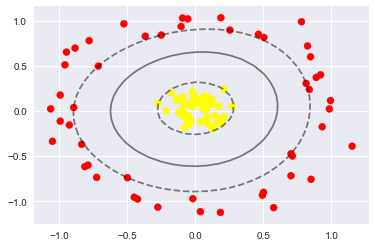
\includegraphics[width=0.45\linewidth]{figures/svc.png}
	\caption{}
	\label{fig:kernel}
\end{figure} 
	
 Most real life cases are not linearly separable, but sometimes we can transform the features hoping that the new features can be separated  with hyper planes. On the image \ref{fig:kernel} we add a third coordinate to the data, the distance to the origin. Then in $R^3$ it is easy to find a plane $z=.6$ that classifies our data. SVM perform better if we pre-process the data following the rules on the notebook ``Cleaning data''. 
 
How can we use this algorithm to find anomalies in new products? we can assume that good products have label 1 and products that are outliers have label 0. By training the SVC this way, it will learn to classify products are regular or outliers. It will recognize when a new product is far from the standard as in fig \ref{fig:novelty}. This idea is explained in the notebook ``SVC II''. 
	
	\begin{figure}[h!]
		\centering
		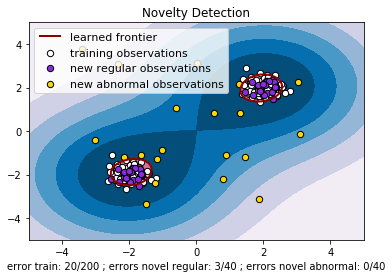
\includegraphics[width=0.45\linewidth]{figures/novelty.png}
		\caption{}
		\label{fig:novelty}
	\end{figure} 
	
% Needed:	Brief description of good and bad points of SVM 
	\subsection{Neural Networks}  
	
	What if instead of using lines or hyperplanes, we use non linear functions to classify our data? A neural network is an improvement over SVM, in the sense that the last component (layer) of a Neural Network behaves like a SVM.
	
	 A neural network is a combination of  functions of the form:
	$x\rightarrow \sigma(W_{a,b}x)$ where $x\in R^b,  W_{a,b}$ is a matriz transformation and $\sigma$ stands for a non linear function applied entry wise to the $a$ coordinates of the vector  $W_{a,b}x.$
	It is standard notation to represent matrices  $W_{a,b}$ as arrows from a column with $b$ neurons to a column with $a$ neurons as in \ref{fig:nn}. Note that in principle some activations could be the identity. If all activations are the identity we can use composition of matrix and reduce the algorithm to SVM. Finding the coefficients of those matrices requires multivariable calculus and relabeling the chain rule. In ``L5 Neural Networks'' you can find an introduction to Keras, which we consider the most friendly language to use Neural Networks, and a deeper explanation of how Neural Networks work and can be trained.	
	
	An important research question is: What determines the architecture of a Neural Network.  The paper "Why does deep and cheap learning work so well?" targets that question from the Physics point of view.
	
	
	An application of Neural Networks to chemistry is contained in the note ``Poterntial Energy Surface ANN'' where we describe the work of The Roitberg group in University of Florida, a transferable deep learning potential based on Belher and Parrinello symmetry functions that is applicable to complex and diverse molecular systems well beyond the training data set: ANAKIN-ME (Accurate NeurAl networK engINe for Molecular Energies) or ANI for short.
	
    	\begin{figure}[h!]
    	\centering
    	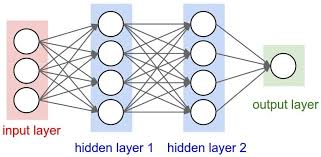
\includegraphics[width=0.45\linewidth]{figures/nn.jpg}
    	\caption{}
    	\label{fig:nn}
    \end{figure} 	

    ``Recurrent Neural Networks'' deals with networks designed for modeling time series data.  Mathematically, our data might be written as $w⋅x^i+w̃ ⋅y_{i−1}$ where  $w$  is the vector containing the weights associated wtih the current inputs  $x^i$  and  $w̃$  is the vector containing the weights of the outputs of the previous time steps  $y_{i−1}$. We are a little bit sloppy with the terminology, the outputs don't necessary have to be from the output layer.
This can be use to make numerical simulations of partial differential equations and ordinary differential equations, and we include an example with pytorch of Character-Level classification of names in ``RNN II''.

    ``Generative Adversarial Networks'' describes a generative method. Suppose that we have a set of examples and we want to generate more images which look like the previous examples. For example, we might have the set of fashion MNIST and we want to generate fake cloths. Or maybe we want to create fake news. Presently known applications are Image denoising, Inpainting, Super-resolution, Structured Prediction, Exploration in Reinforcement Learning and Neural Network Pretraining.

	\subsection{CNN}
	
	Given a picture of an Warehouse Shelving, a  neural network can immediately identify the objects and add them to the inventory. Chinese government used face recognition to identify fugitives in a music concert. It is possible to train a special Neural Network called Convolutional Neural Network, to transfer the style of a paint into a different paint as we will see in ``Style Transfer'' and `` Pix2Pix'', see fig \ref{fig:botero}. 
	
	
	\begin{figure}[h!]
		\centering
		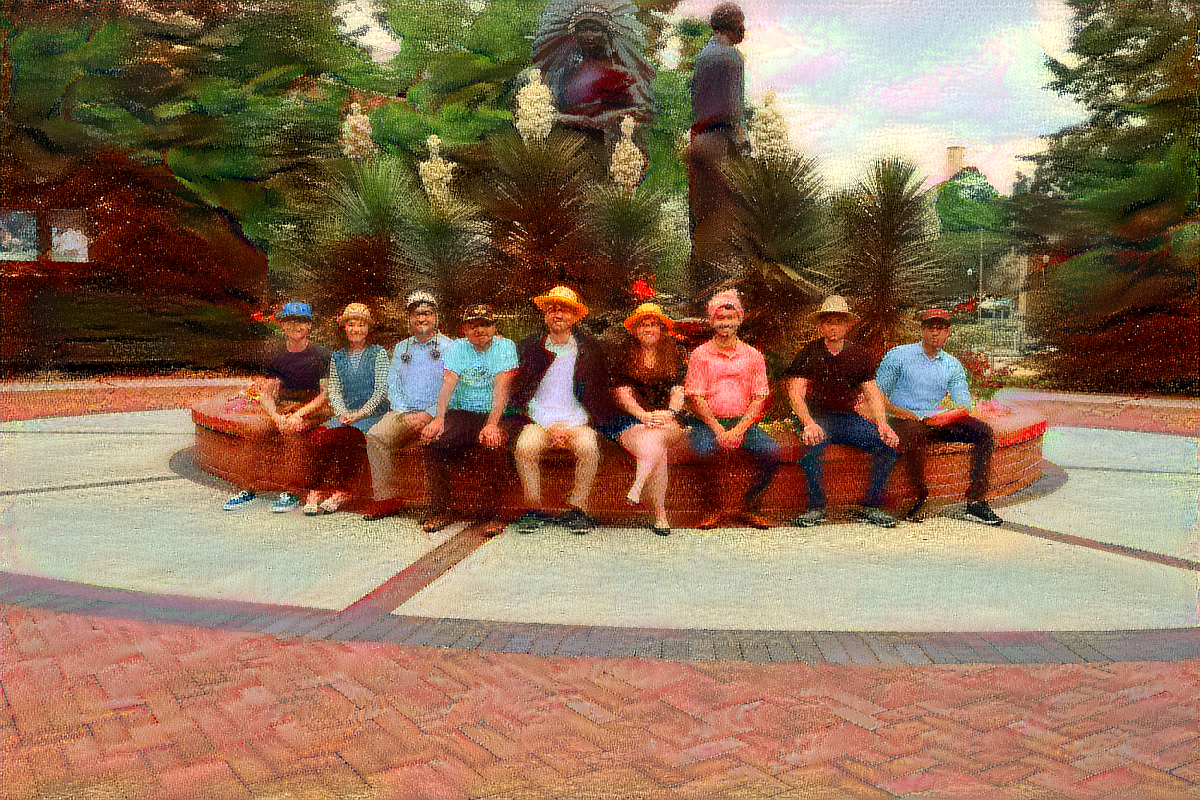
\includegraphics[width=0.45\linewidth]{figures/botero.png}
		\caption{}
		\label{fig:botero}
	\end{figure} 	
	
	The main problem with images, is that they are represented as vectors that are too large. Go to your favorite browser and look for images with exactly  $500\times500$ pixels. That is $250000\times3$ numbers. Normal Neural Networks will require you to find too many matrix coefficients. Besides that, we are not working any more on the case $R^b\rightarrow_{ M_{a,b}} R^a$ as the pixels are related with the pixels in their neighborhood, including pixels above and below, so we want to use this information, which may be missing if we just think of an image as a very long vector. 
	 
	
	We need to change the vectors input to matrices input,  and the vectors output to matrix output. You can think of a matrix as a vector with vector entries.  So now the matrices are not only operations but the elements we work on.
	Instead of learning a coefficient of a matrix, we learn a filter. The good thing of image processing is that we have visual help to understand the process. A filter may be geometric information that is present in several parts of the image, as the concept of a curve, or a square, see fig \ref{fig:filter} .  
	
	\begin{figure}[h!]
		\centering
		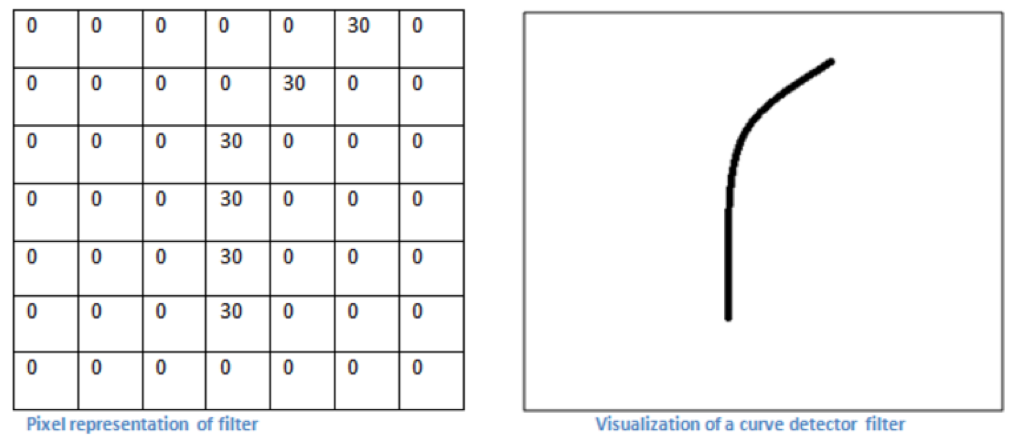
\includegraphics[width=0.45\linewidth]{figures/filter.png}
		\caption{}
		\label{fig:filter}
	\end{figure} 	

	
	In ``CNN'' we explain in more detail how CNN work. In lecture ``Deep Dreams" we ask the neural network if it recognizes a pattern and then we modify images to show that pattern. In `` Style transfer'' we learn images styles and impose them to other images, for example  in \ref{fig:botero} we used a picture of our team and we added the style of a paint of Botero. %Lecture "L 25" is TBD.
	
	
\subsection{Bayesian methods}
In ``Frequentist vs Bayes''
 we introduce Bayesian methods and show how do they differ from the frequetist perspective. 
 
Frequently we want to quantify the accuracy of our predictions. In the ``Markov'' lectures we find a Bayesian approach--one where we consider the values of the parameters as random variables is a popular method.

Recall Bayes' theorem for training parameters
\begin{equation}
P(\theta|X_{train}, T_{train}) = \frac{P(T_{train}, \theta|X_{train})}{\int P(T_{train}, \theta|X_{train})\;\mathrm{d}\theta} 
\end{equation}

The integral on the bottom is generally not analytic. And for higher dimensional problems, infeasible to calculate. By using Monte Carlo Markov Chain algorithm, it is possible to make estimations.  This is also useful to study   the Ising model, which was created to describe Magnetic and ferromagnetic materials. We also introduce Simulated Annealing and Uncertainty Quantification.

After this notebook,  we recommend to read ``Why does deep and cheap learning work so well?''.  The authors use physics to train to explain the way neural networks are capable to make classifications. 
\subsection{Genetic Algorithms}
A genetic algorithm is a search heuristic  inspired by Charles Darwin’s theory of natural evolution. They reflect the process of natural selection where the fittest individuals are selected for reproduction in order to produce offspring of the next generation.



Genetic Algorithms are most commonly used in optimization problems wherein we have to maximize or minimize a given objective function value under a given set of constraints. GAs are also used to characterize various economic models like the cobweb model, game theory equilibrium resolution, asset pricing, etc. They also have been used to plan the path which a robot arm takes by moving from one point to another. We can find more applications in multimodal optimization in which we have to find multiple optimum solutions.



\begin{figure}[h!]
	\centering
	\includegraphics[width=0.45\linewidth]{figures/GAfigure1.png}
	\caption{}
	\label{fig:GA}
\end{figure} 	


Given a problem we define a fitness function that measures how good is a proposed solution. The higher the fitness the closer to an ideal solution of my problem.
The process of natural selection starts with the selection of fittest individuals from a random population, we also select a percentage of the remaining population. This new smaller population produce offspring, mixing genes that seem useful to solve our problem. To explore new genes, we mutate a small percentage of the offspring and add foreigners to obtain the new population.

By doing this process several times, the maximum value obtained by the fitness function on the population cannot  decrease as every new generation has the fittest individuals of the previous generation, while the mutations and foreigners help us avoid fixed points that are not minimums. 

Advantages of Genetic Algorithms. They does not require any derivative information (which may not be available for many real-world problems). They have very good parallel capabilities. They always give an answer to the problem, which gets better over the time.
Useful when the search space is very large and there are a large number of parameters involved.

Limitations. GAs are not suited for all problems, especially problems which are simple and for which derivative information is available. Probably we don't get the global optimum solution. Fitness value is calculated repeatedly which might be computationally expensive for some problems.
Being stochastic, there are no guarantees on the optimality or the quality of the solution.
If not implemented properly, the GA may not converge to the optimal solution.
		
For more details see the notebook ``Genetic Algorithm'' and the notebook ``GARFfield'' where an application to reactive force fields is explained.
 
	 \subsection{Decision Trees}
 We think of a feature as a vertex of a tree, and we think of the possible values of that feature as branches. The order in which we choose the features give us different shapes of trees. Among those trees, we argue that trees with low entropy are better for classification, you can find an algorithm in the notebook ``Decision Trees'' to build your decision tree.


\begin{figure}[h!]
	\centering
	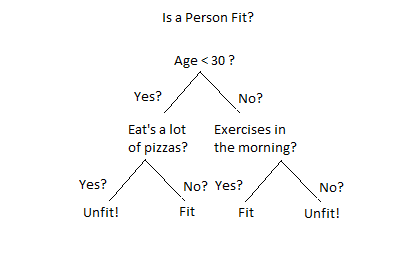
\includegraphics[width=0.45\linewidth]{figures/Decision-Trees.png}
	\caption{}
	\label{fig:Trees}
\end{figure} 	
Advantages of decision trees:
They are simple to understand, they can handle both numerical and categorical data, they are relatively little data preparation needed, the mechanism for the model can be easily extracted and understood, they are robust against co-linearity.

 Disadvantages: Accuracy, they tend to overfit, and the locality of optimization.
 
 
 \subsection{KNN}
 In K-Nearest-Neighbors, we make a prediction or classify an element by  only analyzing  a neighborhood of the element.  Basic Idea:
 
 1.- Get some example set of cases with known outputs. (Diagnosis of diseases.)
 
 2.-When you see a new case, assign its output to be the same as the most similar known case. (Your simptomes resemble Mr. T, Mr. T has the flu, Ergo you have the flu).

 $K$ stands for how many points nearby do you consider to make your choice. Given a new point $x$ and the closest $k$ points to $x$, you can assign to $x$ the average of $x$'s neighbors values. Here the results depend on a good choice of the parameter $K$. This method gives bad approximations on the boundary. If the boundary is a concern,  Kernel Regression assigns different weights to the nearby points so that points that are closer matter most. 
 
 Locally weighted polynomial  regression is a local version of polynomial regression.
 The possibility to write a model that deals with the local picture is important in applications as we will see at the end of this section.
 
 \begin{figure}[h!]
 	\centering
 	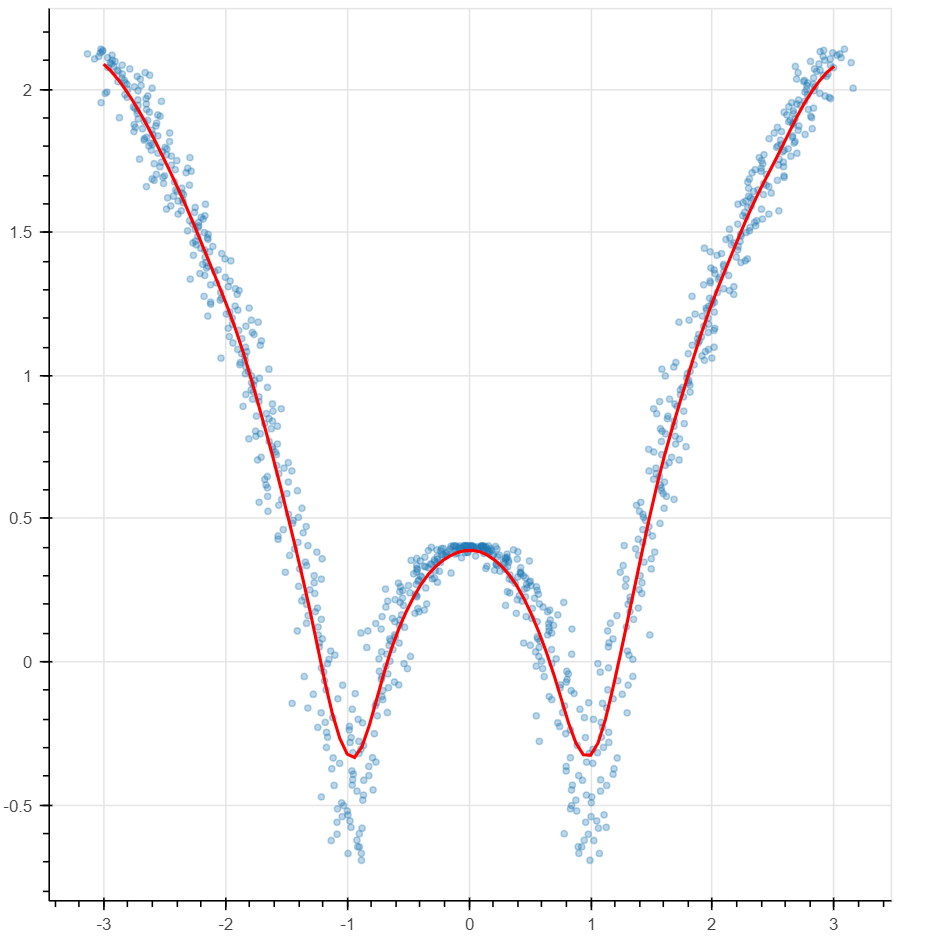
\includegraphics[width=0.45\linewidth]{figures/bokeh_plot.png}
 	\caption{}
 	\label{fig:knn}
 \end{figure} 	
 In this notebook we deal with  memory based algorithms, 
 they are all easy to adapt to new training samples, so there is no need to retrain them. They 
 can handle complex decision boundaries and functions by considering the query instance when deciding how to generalize.
 The cons are that they require retaining all training examples in memory, so it is slow to evaluate a new query and the evaluation time grows with the dataset size.
  
Using local polynomial linear regression we will reproduce a typical diagram in phase transition.
 \begin{figure}[h!]
	\centering
	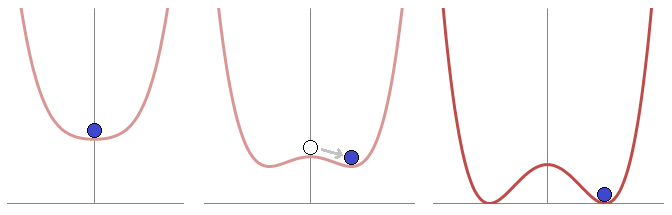
\includegraphics[width=0.45\linewidth]{figures/image.png}
	\caption{The 3d mexican hat potential.} 
	\label{fig:face}
\end{figure} 	
Let's look at figure \ref{fig:face}. It shows a the ball rolling spontaneously to one side of a 2D W-graph. Let's think of this graph as some sort of potential, which is physics for energy function.

We can think of the ball settled at the bottom of the parabola as the ground-state of the "high temperature" or "high energy" regime of some system. 

This ground state, the ball at the bottom of the parabola, is a unique ground state. 

By this we mean there is a SINGLE state of the system, where if we were to rotate the system about the Z-axis (axis running through center of parabola), the energy of the system would not change. We call this system $U(1)$ symmetric. 

Now consider the low-energy or low-temperature regime: the ball has settled into either side of the quartic-graph. 

In this regime, there is no longer a unique ground state, the ball being on the left or on the right are configurations that correspond to the same energy values. Therefore, we say there is a DEGENERACY of the ground states, and there is no way to distinguish one configuration from the other simply in terms of energy. We call this parity symmetry. Although our low-energy system has "broken the symmetry" of $U(1)$ by falling into the left or right side. These two sides have the same energy and are thus indistinguishable. This means we can call them parity invariant. This parity invariance is characterized by a group of transformations of the ground state that leave the energy unchanged. It turns out that this group of transformations is the group of rotations of the "phase" of the system. 




\subsection{SOM}
 \subsection{Cocktail party problem}
 \subsection{Non Negative Tensor Factorization}
 
We consider data in form of a matrix. For example, given a vocabulary with  m  words, and  n  documents,  $V_{ik}$ is  the number of times the  $i$ -word in the dictionary appears on the  $k$  document.
A database of gray-scale images of a fixed size can also be described by a matrix $V$.  We relabel the pixels in an image form $1$ to $ m$, and assume the  database has $n$ images. The value of the $V_{ik}$ is the intensity of the $i$-pixel in the $k$ image. 

Non negative matrix factorization is a process to find two matrices with non negative entries $W,H$ so that $V\sim W\times H$. It turns out that the columns of $H$ can be understood as a basis whose linear combination approximates the columns of $V$. $W$ give us the coefficients so that a juxtaposition of the columns of  $H$ can recover the initial data. Columns of $H$ have been recognized as eigen images. This method is used in topic selection.  
 
 

Imagine that for every patient you have a matrix of diagnosis and medications. We can put the column of medications and the rows of diagnosis. So the entries will be mostly zeroes, except when the patient was diagnosed with the $i$-sickness and received the $k$-medication. If we consider a third dimension given by the patient, then we have a 3-dimensional matrix or a vector.
 There is a higher dimensional version of tensor factorization  where we substitute  matrices by tensors. 
 The main yoga was that the non negativity constrain allow us to recover the initial object from juxtaposition of it's parts. 
 When we  replaced matrices by tensors we substitute the factorization into matrix multiplication by tensor decomposition into rank one tensors. 
 
 
In Medicine, Tensor decomposition into rank one tensor shows concurring diagnosis and medications, this process is known as phenotyping.  The study of tensors (phenotypes) using machine learning lead to the discovering of 3 distinct groups of Hearth Failure with preserved Ejection Fractions (HFpEF), those groups 'differed markedly in clinical characteristics, cardiac structure/function, invasive hemodynamics, and outcomes'.
 
 

		%should we include reaction networks??????
			
		
		

	
	
	
	%%*************************************************************** %
	%% % % % % % % % % % % % % % % % % % % % % % % % % % % % % % % % %
	%%*************************************************************** %
	%%*************************************************************** %
	%% % % % % % % % % % % % % % % % % % % % % % % % % % % % % % % % %
	%%*************************************************************** %
	%%*************************************************************** %
	%% % % % % % % % % % % % % % % % % % % % % % % % % % % % % % % % %
	%%*************************************************************** %
	
	%%%%%%%%%%%%%%%%%%%%%%%%%%%%%%%%%%%%%
	%% Begin Chapter Document %%%%%%%%%%%%%%%%%%%%%
	%%%%%%%%%%%%%%%%%%%%%%%%%%%%%%%%%%%%%
	
	\chapter{Results}
	
	
	%%*************************************************************** %
	%% % % % % % % % % % % % % % % % % % % % % % % % % % % % % % % % %
	%%*************************************************************** %
	%%*************************************************************** %
	%% % % % % % % % % % % % % % % % % % % % % % % % % % % % % % % % %
	%%*************************************************************** %
	%%*************************************************************** %
	%% % % % % % % % % % % % % % % % % % % % % % % % % % % % % % % % %
	%%*************************************************************** %
	
	%%%%%%%%%%%%%%%%%%%%%%%%%%%%%%%%%%%%%
	%% Begin Chapter Document %%%%%%%%%%%%%%%%%%%%%
	%%%%%%%%%%%%%%%%%%%%%%%%%%%%%%%%%%%%%
	
	
	\chapter{Conclusions}
	Here we will put the most significant results over time
	
	
	%*************************************************************** %
	% % % % % % % % % % % % % % % % % % % % % % % % % % % % % % % % %
	%*************************************************************** %
	%*************************************************************** %
	% % % % % % % % % % % % % % % % % % % % % % % % % % % % % % % % %
	%*************************************************************** %
	%*************************************************************** %
	% % % % % % % % % % % % % % % % % % % % % % % % % % % % % % % % %
	%*************************************************************** %
	
	%%%%%%%%%%%%%%%%%%%%%%%%%%%%%%%%%%%%
	% Begin Appendix Chapter Document %%%%%%%%%%%%%%%%%%%%%
	%%%%%%%%%%%%%%%%%%%%%%%%%%%%%%%%%%%%
	
	\appendix
	\addcontentsline{toc}{chapter}{Appendix}
	
	\chapter[Scripts]{Scripts}
	
	\chapter{Extra plots}
	
	\chapter{Inputs}
	
	
	%%%%%%%%%%%%%%%%%%%%%%%%%%%%%%%%%%%%
	% Begin Appendix Bibliography Document %%%%%%%%%%%%%%%%%%%%%
	%%%%%%%%%%%%%%%%%%%%%%%%%%%%%%%%%%%%
	
	\bibliographystyle{unsrt}
	\bibliography{../Papers_related/pfmg}
	
	
\end{document}


